
\chapter{Introduction}

\section{Transcriptional Regulation}

In 3.5 billion years, evolution has tinkered with life on Earth and several
cellular mechanisms have evolved for living things to sense and react to
ever-changing conditions in their environment, such as temperature, nutrient
availability or presence of toxic compounds. The fundamental way for organisms
to respond to such environmental changes at the cell level by regulating
gene expression: controlling the production rate of gene products.

There are a variety of mechanisms to control gene expression at different
levels of gene product synthesis, such as the regulation of transcriptional
initiation, post-transcriptional RNA interference, and post-translational
proteolysis~\cite{snyder2007molecular}. Genomic features such as gene copy
number, guanine-cytosine (GC) content, and codon usage patterns also affect the
regulation of gene expression~\cite{gustafsson2004codon,
  stranger2007relative}. Probably the most common mechanism employed by all
cellular systems is the regulation of transcriptional
initiation~\cite{browning2004regulation}. This is not surprising, because
regulation of transcription initiation is the most economical way for a cell to
control the expression level of its genes~\cite{malacinski2005essentials}. The
mechanisms at the pre-transcriptional level cannot be flexible since they would
require changes in the genome. On the other hand, any mechanism following the
transcription would be a waste of already produced messenger RNA (mRNA)
transcripts.

DNA-binding proteins, called transcription factors (TF), play the central role
in the regulation of transcription initiation. A TF activates or represses
transcription initiation of a gene by assisting or blocking the binding of RNA
polymerase to its promoter region~\cite{reznikoff1985regulation}. A TF
recognizes and binds to specific DNA sequences, called transcription factor
binding sites (TFBS), that are of length 10--20 bp~\cite{gerland2002physical,
  berg2004adaptive} and mostly located between -60 and +60 base pairs (bp)
relative to the transcriptional start site~\cite{collado1991control}. This set
of similar, but not identical, TF binding sites describes the binding pattern
that the TF looks for binding, known as transcription factor binding motif. An
example of sequences recognized by TF, the binding sites of the hypothetical
protein Hyp is given in Table~\ref{tab:lexa-motif}.

\begin{table}[h]
  \centering
  \caption{Collection of binding sites for the hypothetical protein Hyp.}
  \label{tab:lexa-motif}
  \begin{tabular}{c}
\texttt{AGGTAAACCT}\\
\texttt{CCGTAAACCT}\\
\texttt{AGGTTGACCG}\\
\texttt{CAGTCAACGG}\\
\texttt{AGGTCACCAT}\\
\texttt{AGGTACACTT}\\
\texttt{TGGTAAACCA}\\
\texttt{AGGTATCCCT}\\
\texttt{GTGTGACACT}\\
\texttt{AGGTAACCAA}\\
\texttt{AGGTATACCT}\\
\texttt{TGGTAAACCA}\\
\texttt{CAGTCAACGG}\\
\texttt{AGGTATACCT}\\
\texttt{TGGTAAACCA}
   \end{tabular}
\end{table}


\subsection{Representation of TF binding motifs}

The classical representation of a binding motif is the consensus sequence, the
sequence of the most frequent base at each position of the aligned binding
sites~\cite{pierce2012genetics}. The consensus sequence for the binding motif
in Table~\ref{tab:lexa-motif} is \texttt{AGGTAAACCT}. Although consensus
sequences are widely used in molecular biology, and they describe the binding
motif in a very simple way, they have flaws due to this very
simplicity~\cite{schneider2002consensus}. For example, a column that contains
an adenine most of the time is represented by an A, but the consensus sequence
does not say anything about the frequency of bases. It is equally likely that
the position might contain 95\% A or it could have 51\% A and 49\% T. The
problem occurs when one looks for additional binding sites using the consensus
sequence.  If no mismatch is allowed, almost half of acceptable sequences could
be missed in the case of 51\% A and 49\% T. For example, -10 region of
bacterial promoters has the consensus sequence \texttt{TATAAT}, also known as
Pribnow box~\cite{pribnow1975nucleotide}. However,  very few promoters
contain the exact consensus sequence~\cite{lisser1993compilation}. Even when
mismatches are allowed, allowing a mismatch in a very well-conserved column
is equivalent to allowing a mismatch in a position that is not
conserved. A better representation of the binding motif that captures more
information is known as Position Specific Frequency Matrix (PSFM).

A PSFM is a $4 \times L$ matrix, containing one row for each base and one
column for each position of the alignment. Each entry of the PSFM, $f_{i, j}$,
is the observed relative frequency of the base $i$ in $j$th column of the
alignment:

\begin{equation}
  \label{eq:psfm}
  f_{i, j} = \frac{n_{i, j}}{\displaystyle\sum_{k=1}^A n_{k, j}}
\end{equation}
where $n_{i, j}$ is the number of occurrences of base $i$ in position $j$ and
$A$ is the alphabet size ($A=4$ for DNA sequences). The PSFM for the
hypothetical motif in Table~\ref{tab:lexa-motif} is given in
Table~\ref{tab:psfm}.

\begin{table}
  \centering
  \caption{The Position Specific Frequency Matrix for hypothetical protein Hyp.}
\label{tab:psfm}
  \begin{tabular}{|r|r|r|r|r|r|r|r|r|r|r|}
\hline
  &    1 &   2 &    3 &    4 &    5 &    6 &    7 &    8 &    9 & 10\\
\hline
A & 0.53 & 0.13 & 0.00 & 0.00 & 0.67 & 0.67 & 0.73 & 0.07 & 0.13 & 0.27 \\
\hline
C & 0.20 & 0.07 & 0.00 & 0.00 & 0.20 & 0.07 & 0.27 & 0.93 & 0.67 & 0.00 \\
\hline
G & 0.07 & 0.73 & 1.00 & 0.00 & 0.07 & 0.07 & 0.00 & 0.00 & 0.13 & 0.20 \\
\hline
T & 0.20 & 0.07 & 0.00 & 1.00 & 0.07 & 0.20 & 0.00 & 0.00 & 0.07 & 0.53 \\
\hline
  \end{tabular}
\end{table}

Given a binding site of length $L$, the odds of it being a functional binding
site can be calculated by first transforming the PSFM into a Position Specific
Weight Matrix (PSWM), also known as Position Specific Scoring Matrix
(PSSM). Each entry of the PSSM is defined as

\begin{equation}
  \label{eq:pssm}
  \mathrm{PSSM}(i, j) = \log_2\left(\frac{f_{i, j}}{p_i}\right)
\end{equation}
where $p_i$ is the background probability of observing base $i$. The PSSM for
the hypothetical motif is given in Table~\ref{tab:pssm}.

\begin{table}
  \centering
  \caption[The Position Specific Scoring Matrix for the hypothetical
  protein.]{The Position Specific Scoring Matrix for the hypothetical protein
    Hyp. A $10^{-100}$ pseudocount is added to all frequencies to avoid
    $\log(0)$ computations. This leads to -334.10 values
    instead of $-\infty$.}
  \label{tab:pssm}
  \begin{tabular}{|r|r|r|r|r|r|r|r|r|r|r|}
\hline
  &     1 &   2 &    3 &    4 &    5 &    6 &    7 &    8 &    9 & 10\\
\hline
A &  1.09 & -0.91 & -334.10 & -334.10 &  1.42 &  1.42 &  1.55   & -1.91 & -0.91&   0.09\\
\hline
C & -0.32 & -1.91 & -334.10 & -334.10 & -0.32 & -1.91 &  0.09   & 1.90  & 1.42 & -334.10\\
\hline
G & -1.91 &  1.55 &  2.00   & -334.10 & -1.91 & -1.91 & -334.10 & -334.10 &  -0.91 & -0.32\\
\hline
T & -0.32 & -1.91 & -334.10 &  2.00   & -1.91 & -0.32 & -334.10 & -334.10 &  -1.91 &  1.09\\
\hline
  \end{tabular}
\end{table}

\subsection{Information content of TF binding motifs}

By applying Shannon’s information theory~\cite{shannon1948mathematical} to TF
binding motifs, entropy, the uncertainty of observing any particular base in
the genomic background is defined as:

\begin{equation}
  \label{eq:hg}
  H_g = -\displaystyle\sum_{i=1}^A p_i \log_2(p_i)
\end{equation}
Similarly, the uncertainty of observing any particular base in a column $j$ of
the alignment is defined as:

\begin{equation}
  \label{eq:hm}
  H_m(j) = -\displaystyle\sum_{i=1}^A f_{i, j} \log_2(f_{i, j})
\end{equation}
Putting together these two uncertainties, the information content (IC) of a
position is defined as the decrease in uncertainty by observing a particular
base in that position~\cite{schneider1986information}.

\begin{equation}
  \label{eq:rseq}
  R_{seq}(j) = H_g - H_m(j)
\end{equation}
And finally, assumping positional independence, the total IC of the motif is

\begin{equation}
  \label{eq:1}
  R_{seq} = \displaystyle\sum_{i=1}^L R_{seq}(j)
\end{equation}
where $L$ is the motif length.

Sequence logos are a commonly used graphical representation of binding
motifs~\cite{schneider1990sequence, crooks2004weblogo}. A sequence logo
represents each column of the motif with a stack of letters such that the
height of the stack is the information content of the column whereas the
relative heights of each letter in the column represents their relative
frequencies. The sequence logo for the hypothetical protein with the binding
motif in Table~\ref{tab:lexa-motif} is given in Figure~\ref{fig:lexa}.

\begin{figure}
  \centering
  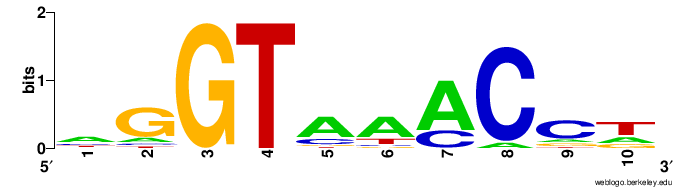
\includegraphics[width=0.6\textwidth]{figures/chapter1/hyp.png}
  \caption{The sequence logo for the hypothetical protein Hyp.}
  \label{fig:lexa}
\end{figure}

\section{Evolution of Transcriptional Regulatory Elements}

The interaction between a TF and its binding sites is essential for
regulation. To maintain the regulatory interaction, a mutation in one of these
elements (i.e. TF and its binding sites) must be counterbalanced by a change in
the other element. This co-evolution between TFs and their binding motifs has
been observed for eukaryotic TFs~\cite{yang2011correlated}. In closely related
Bacteria, it has been shown that orthologous TFs, the products of genes that
evolved from a common ancestor by speciation, tend to have conserved binding
motifs~\cite{makarova2001conservation}. Although this tendency has been
observed among more distant Bacteria for some TFs (e.g. ArgR/AhrC and HrcA
regulating arginine metabolism~\cite{maas1994arginine, klingel1995binding}), it
does not hold for some other TFs such as SOS response regulator LexA in
Gram-negative Bacteria~\cite{walker1985inducible} and DinR, its ortholog in
Gram-positive Bacteria~\cite{winterling1998bacillus}.

Another aspect of the evolution of transcriptional regulatory elements is the
co-evolution between the TF and its regulon. Conservation of regulons has been
observed across closely related genomes having orthologous
TFs~\cite{mironov1999computer, tan2001comparative}. Another study reported
conservation of the overall function in the regulon controlled by orthologous
TFs, despite pervasive gain and loss of target genes, in
eukaryotes~\cite{habib2012functional}. Interestingly, it has also been
suggested that, among distantly related Bacteria, orthologous TFs may have
different functions and regulate different
genes~\cite{price2007orthologous}. Finally, it has also been suggested that
transcriptional regulatory networks (TRN) are highly dynamic, whereas TFs tend to
be more conserved~\cite{babu2006evolutionary, chavez2006bacterial}.

\section{Comparative Genomics}

Since the whole genome sequencing of two bacterial species, \textit{Haemophilus
  influenzae} and \textit{Mycoplasma genitalium}~\cite{fleischmann1995whole,
  fraser1995minimal}, comparative genomics has become a standard tool to
analyze evolutionary relationships among species. It has been used many times
to characterize transcriptional regulatory networks and to investigate their
evolutionary relationships across different
Bacteria~\cite{gelfand2000prediction, ravcheev2013genomic,
  meireles2009comparative, kellis2004methods, erill2004differences,
  erill2007aeons, sanchez2012analysis, cornish2012inference}.

A conventional comparative genomics analysis of a TRN starts with the transfer
of available information on the regulatory network (TF-binding motif and
regulated genes) to the species under analysis to infer the binding motifs in
these target species. The following step is the genome-wide search in target
genomes using their inferred TF-binding motifs. A TF-binding model, such as the
PSSM, is used to scan target genome sequences to identify high scoring sites. The
third and final step is the integration of search results from multiple genomes
to validate putative sites identified in the previous step. This aggregation of
results reduces the number of false positives dramatically by assuming that
only orthologs of regulated genes will systematically display TF-binding sites
in their promoters whereas false positives should be randomly scattered across
genomes~\cite{rodionov2007comparative}.


\section{Statement of the Problem}

The advances in the molecular biology technologies pose new challenges for
bioinformatics. New technologies that shift the nature and amount of
experimental data require improvements on existing datasets compiled using
traditional data collection process, and methods performing on these datasets.

The high-throughput technologies such as ChIP-Seq~\cite{bailey2013practical}
have increased the amount of TF binding data tremendously. However, the
increasing amount of the available experimental TFBS data challenges the
underlying definition and the collection process of TF-binding site
data~\cite{salgado2013regulondb}. Although there are well-established
eukaryotic TF-binding site databases~\cite{mathelier2015jaspar,
  matys2003transfac}, their counterparts in Bacteria domain are mostly
organism-specific~\cite{salgado2013regulondb, sierro2008dbtbs,
  jacques2005mtbreglist, pauling2012coryneregnet}. Some of these databases have
not been updated in several years, thereby missing huge amounts of
data~\cite{munch2003prodoric}. Also, these databases often mix experimentally
validated sites with computationally predicted
ones~\cite{kazakov2007regtransbase}, introducing biases in the machine learning
and comparative genomics techniques that depend on them to model TF-binding
site interactions. Closing the circle, the putative binding sites identified by
these biased methods are captured by the databases and mixed with the
experimentally-verified ones, introducing further bias.

Comparative genomics can leverage the vast amount of genomics sequences to
reconstruct and analyze TRNs in Bacteria, but its efficacy hinges on the
ability to transfer regulatory networks from reference species to the genomes
under analysis. Several methods have been proposed to transfer regulatory
information between bacterial species~\cite{babu2009methods,
  baumbach2010power}, but the paucity and distributed nature of experimental
data on bacterial transcriptional networks have prevented their systematic
evaluation so far.

Using the existing limited datasets and methods for reconstruction of the TRNs
that have not been evaluated, comparative genomics analysis tools suffer from
the problems associated with them. They provide semi-automatic workflows that
have been reported to work well in some cases, yet they lack systematic
evaluation using existing data. Another problem with existing tools is their
limitation to a set of preprocessed genomes. To avoid the dynamic computation
of some features required for comparative analysis, such as ortholog detection,
they restrict the user to a large yet still limited and irregularly updated
collection of genomes. Therefore, they are not suitable for TRN analysis of
recently sequenced and annotated genomes that are being added to central
sequence databases such as NCBI RefSeq~\cite{o2015reference} every
day. Furthermore, binding site predictions are usually reported with raw scores
(e.g. PSSM scores), requiring the user to predefine a threshold to determine
what constitutes a putative binding site. Setting a threshold, however,
necessitates knowledge about the TRN of the genome under analysis, the very
thing that the analysis is performed for. Finally, the lack of ancestral state
reconstruction methods integrated with the existing platforms make difficult
formally to reconstruct the evolutionary history of the TF regulation based on
available data.

In summary, this dissertation addresses three major issues of existing
comparative genomics workflows.

\begin{enumerate}
\item Existing TFBS databases do not capture prokaryotic-wide up-to-date
  binding site data and do not clearly separate experimentally validated and
  computationally predicted binding sites. Some of them do not contain any data
  from the last few years, missing a significant portion of existing TF-binding
  information. Also, their lack of integration with major sequence databases
  threatens the availability of the compiled data in the future.

\item As the first step of comparative genomics of TRNs, there have been
  several methods employed and reported to perform well for transferring
  available TFBS and regulon information to genomes of interest. Partly due to
  lack of compiled data, their performance on identifying TF binding motif and
  TRN in target species has never been systematically evaluated.

\item The few existing comparative genomics platforms for TRNs adopt
  methodologies that have not been evaluated. They limit usage to preprocessed
  genomes which often do not include recently sequenced and annotated
  genomes. They usually report raw scores for predictions, making difficult to
  assess the confidence level of each prediction.  Finally, apart from
  identifying orthologous groups of regulated genes, they lack any methods to
  integrate reconstructed TRNs of all genomes under analysis, such as inferring
  the regulatory state in ancestral species, which is essential to reconstruct
  the evolutionary history of TF regulation.
\end{enumerate}

\section{Research Design}

The main goal of this study is to design and develop a full comparative
genomics pipeline, addressing the shortcomings of the previous attempts at all
levels of the workflow which are (1) collection of experimentally validated
TFBS data, (2) assessment of existing motif and regulon transfer methods and
(3) development of a general-purpose comparative genomics tool for TRN
analysis.

\textit{Development of a prokaryotic-wide TFBS database.}
Experimentally verified TFBS data, available in organismal databases or not
curated at all, needs to be compiled. To enforce high quality on the data, only
binding sites with experimental evidence showing TF binding and gene expression
should be curated and inserted into the database. The data should be supported
with the metadata such as the publication information and experimental methods
used to validate binding. Also, the data should be easily browsable, allowing
access to TF-binding motifs of particular TF-species pairs confirmed with
specified experimental techniques, as well as integrating TFBS data from
multiple species (e.g. LexA binding sites in all Firmicutes). Also, the
developed database should integrate the data with major biological sequence
resources to ensure the availability of the curated information in the long
term.

\textit{Benchmarking of TF binding motif and regulon transfer methods.}
Existing TF-binding motif and regulon transfer methods need to be evaluated by
measuring their accuracy to transfer known motif and regulon in reference
species and infer true binding motifs in target species. These methods and
their variations need to be tested on the prokaryotic-wide TFBS data compiled
as a part of the first section of this study. Also, the correlation between the
phylogenetic distance of reference and target species, and the accuracy of the
ensuing transfer needs to be investigated.

\textit{Development of a comparative genomics analysis platform.}  By
collecting the data in the first step and using the findings of the assessment
of transfer methods in the second step, a comparative genomics analysis
platform needs to be designed, developed and made available for public
use. In contrast with existing ones, the developed platform should be able to
perform analysis on any annotated genome, and be able to combine
binding evidence from multiple sources (e.g. TFBS collections from different
species). Also, given a promoter of an operon, the platform should not require
the user to decide on a score threshold and merely report PSSM scores higher
than the threshold. Instead, it should be able to incorporate prior belief of
TF regulation (defined by the user or inferred using available data) and the
PSSM scores over the entire promoter region into a posterior probability of
binding, a natural and more interpretable value than PSSM scores. Finally,
rather than just identifying putative binding sites and regulons in all species
under analysis, the platform should implement ancestral state reconstruction,
an integrative method to extrapolate the measured traits (i.e.\ gene
regulation) back in time to common ancestors of target species. Inferring the
regulatory state in ancestral species would help to test evolutionary
hypotheses on TF regulation.

\section{Results}

\textit{Development of a prokaryotic-wide TFBS database.}  The efforts to
capture the interaction of TFs with their target sites led to CollecTF, a
database of TFBS in the Bacteria domain~\cite{kilic2013collectf,
  kilicc2016data}. CollecTF compiles data on experimentally validated,
naturally occurring TFBS across the Bacteria domain, placing great emphasis on
the curation process, the quality and availability of the stored data and fully
customizable access to its records. It integrates multiple sources of evidence
automatically and openly, allowing users dynamically to redefine binding motifs
and their experimental support base. Data quality and currency are fostered by
adopting a sustainable model that encourages direct author submissions in
combination with in-house validation and curation of published
literature. Since its inception, CollecTF has progressively become a portal for
the annotation and submission of information on transcriptional regulatory
elements to major biological resources such as RefSeq~\cite{o2015reference},
UniProtKB~\cite{uniprot2014uniprot}, and the Gene Ontology
Consortium~\cite{gene2013gene}. As a database, it provides enhanced search and
browsing, targeted data exports, binding motif analysis tools and integration
with motif discovery and search platforms.

\textit{Benchmarking of TF binding motif and regulon transfer methods.}
As part of the systematic benchmark of the transfer methods, the motif- and
accuracy-based metrics that assess the results of regulatory network transfer
were evaluated and the precision-recall area-under-the-curve was identified as
the best metric for this purpose due to the class-imbalanced nature of the
problem. Methods assuming conservation of the TF binding motif (motif-based)
were shown to outperform substantially those assuming conservation of regulon
composition (network-transfer), even though their efficiency can decrease
sharply with increasing phylogenetic distance. Variations of the basic
motif-transfer method did not yield significant improvements in transfer
accuracy. The results indicate that detection of a large enough number of
regulated orthologs is critical for network-based transfer methods, but
relaxing orthology requirements does not improve results. Using the
transcriptional regulators LexA and Fur as case examples, it was also shown how
DNA-binding domain sequence similarity can yield confounding results as an
indicator of transfer efficiency for motif-based methods.

\textit{Development of a comparative genomics analysis platform.} Following the
compilation of data and assessment of transfer methods, CGB, a comparative
genomics platform for the analysis of TRNs in Bacteria domain, was
developed. Given a set of TFBS collections from multiple species and a group of
target genomes, CGB builds a PSSM model, adjusted for each target genome by
weighting the evidence from each reference species according to their
phylogenetic distances. It predicts operons on each target genome and scores
their promoter regions using adjusted PSSMs. In addition to identifying binding
sites with high scores, for a given promoter, CGB adopts a Bayesian framework,
combining all positional scores and integrating the prior belief of regulation
into a posterior probability of TF binding to the promoter region and hence putative
regulation of the operon. Following the posterior probability computation for
each operon, CGB identifies orthologous groups of regulated genes and performs
ancestral state reconstruction for each ortholog group to infer the state
(i.e.\ regulation, no regulation or absence of the gene) in common ancestors of
species under analysis. Its utility was demonstrated by performing a
comparative analysis of SOS response regulator LexA in Gram-positive
Bacteria. The CGB is available for public use as a Python library, as well as a
stand-alone tool with a graphical user interface.

\section{Significance of the Study}

The research described in this dissertation aims to improve the entire pipeline
for comparative genomics of bacterial TRNs by collecting data, evaluating
existing methods and developing an automated workflow for reconstructing TRNs
in a group of related Bacteria and their evolutionary analysis.

\textit{Development of a prokaryotic-wide TFBS database.}  By putting a strong
emphasis on collecting only experimentally validated TFBS data, the
high-quality of the stored data facilitates accurate comparative genomics and
machine learning analyses. Also, adopting an open and sustainable model
supports direct author submissions in combination with in-house validation and
curation of the published literature. Integration with major sequence databases
ensures the availability of the data, maximizes its visibility and encourages
direct author submissions.

\textit{Benchmark of TF binding motif and regulon transfer methods.} The
evaluation of metrics to assess the efficiency of methods for transferring TRN
information challenges the established metrics used in the literature. Also,
the compilation of a large catalog of TFBS across Bacteria and its use to
systematically benchmark existing motif and regulon transfer methods is the
first attempt at a domain-wise analysis in the field. The assessment of
transfer methods using the large dataset will enable more informed selection of
transfer methods and, as a result, will result in more accurate comparative
genomics analyses.

\textit{Development of a comparative genomics analysis platform.} The
development of automated yet customizable comparative genomics platform will
enable fast and accurate comparative analysis of TRNs in Bacteria. The ability
of the developed platform to combine and weight TF binding evidence from
multiple species allows using limited TF binding motif data in an efficient
way. Being able to analyze any sequenced genome allows the characterization of
TRNs of newly sequenced genomes of interest. In contrast with the few available
comparative genomics pipelines, the adoption of a Bayesian framework for
reconstructing regulons produces interpretable results. Ancestral state
reconstruction makes it possible to test hypotheses on how the TF of interest,
its binding motifs and regulons might have evolved across species in different
environments.

\section{Assumptions and Limitations}

The need for transferring available regulatory network information from one
species to another stems from the incompleteness of binding site data that
would have allowed comparative analysis directly on experimentally validated
data on each species. Since 2013, CollecTF has compiled over 9,750
experimentally-validated binding sites from over 240 TFs in over 100 bacterial
species. Although it is the largest database of binding sites with direct
experimental evidence only, it is not possible to capture all data for all TFs
and species. First, there is simply not enough studies performed to identify
binding sites experimentally in all species. They mostly focus on particular
TFs and species that have clinical and agricultural importance. The second reason
for the lack of high coverage is the fact that manual curation of each article
is a slow process. Nonetheless, manual curation still produces the highest-quality
knowledge, and this trade-off between the amount of information and its quality
is necessary in order to perform proper machine learning and comparative
genomics analyses.

The most popular model used to approximate specific TF-DNA interactions is the
PSSM\@. A PSSM assumes independence among its different columns. Many studies
have reported that this assumption does not hold true~\cite{man2001non,
  bulyk2002nucleotides, tomovic2007position, osada2004comparative} and others
report that the additive PSSM model is a very good approximation of the
protein-DNA binding~\cite{benos2002additivity}. Despite the arguments on both
sides and the existence of many different types of algorithms including
biophysical models~\cite{stormo1998specificity, djordjevic2003biophysical} and
Hidden Markov Models~\cite{sinha2003probabilistic, drawid2009ohmm,
  salzberg1998microbial}, the PSSM is still the standard model for predicting
binding sites. Although the positional independence assumption can be relaxed
with more complex models~\cite{ben2005identification, zhao2012improved,
  siddharthan2010dinucleotide, barash2003modeling}, the increased number of
parameters introduces the potential for overfitting and requires more data than
is generally available. Consequently, in this study, the PSSM is used to model
binding motifs and to predict binding sites in target genomes.

\section{Organization of the Dissertation}

Chapter 2 describes CollecTF, the database of bacterial TFBS. It starts with
the motivation for creating a new database. Then, the database content and the
curation process is detailed. They are followed by the details on the efforts
of integration with major sequence databases.

Chapter 3 presents a detailed analysis of different methods of motif and
regulon transfer. First, the data compiled from various databases is
described. After that, the metrics for the assessment of transfer methods are
evaluated. The comparison of transfer methods is discussed, and the predictive
indicators of transfer accuracy are analyzed. The chapter ends with the details
of the data and each transfer method used.

Chapter 4 and 5 focus on the comparative genomics analysis of transcriptional
regulatory networks. Chapter 4 describes CGB, the developed comparative
genomics analysis platform. It details each step of the pipeline, from input
processing to visualization and reporting of the results. Chapter 5 studies the
LexA-binding motif of the Verrucomicrobia, a recently established bacterial
phylum of growing interest due to the association of Verrucomicrobia species
with several eukaryotic hosts~\cite{sait2011genomic}, their prominence in many
soil communities~\cite{bergmann2011under} and a significant role in the
adaptability of the human gut microbiome~\cite{dubourg2013high}. In chapter 5,
using CGB, the evolutionary analysis of the SOS response in this phylum is
performed, providing novel insights into the molecular mechanisms driving its
evolution.
